\documentclass[conference]{IEEEtran}
\usepackage{times}

% numbers option provides compact numerical references in the text. 
\usepackage[numbers]{natbib}
\usepackage{multicol}
\usepackage[bookmarks=true]{hyperref}
\usepackage{graphicx}   % need for figures


\begin{document}

% paper title
\title{Robust Combinatorial Planning \\ over Simple Boundary Interactions}

\author{\authorblockN{Alexandra Q. Nilles}
\authorblockA{Department of Computer Science\\
University of Illinois at Urbana-Champaign\\
Email: nilles2@illinois.edu}
\and
\authorblockN{Steven M. LaValle}
\authorblockA{Department of Computer Science\\
University of Illinois at Urbana-Champaign; and\\
Faculty of Information Technology and Electrical Engineering\\
University of Oulu, Oulu, Finland\\
Email: lavalle@illinois.edu}}

%\author{\authorblockN{Michael Shell\authorrefmark{1},
%Homer Simpson\authorrefmark{2},
%James Kirk\authorrefmark{3}, 
%Montgomery Scott\authorrefmark{3} and
%Eldon Tyrell\authorrefmark{4}}
%\authorblockA{\authorrefmark{1}School of Electrical and Computer Engineering\\
%Georgia Institute of Technology,
%Atlanta, Georgia 30332--0250\\ Email: mshell@ece.gatech.edu}
%\authorblockA{\authorrefmark{2}Twentieth Century Fox, Springfield, USA\\
%Email: homer@thesimpsons.com}
%\authorblockA{\authorrefmark{3}Starfleet Academy, San Francisco, California 96678-2391\\
%Telephone: (800) 555--1212, Fax: (888) 555--1212}
%\authorblockA{\authorrefmark{4}Tyrell Inc., 123 Replicant Street, Los Angeles, California 90210--4321}}

\maketitle

\begin{abstract}
Many mobile robots, such as vacuum bots, are now able to move reliably in
straight lines and detect when they have encountered a physical or virtual
obstacle. By planning explicitly over reorientation actions that the robot takes when
encountering a boundary, we may avoid needing to compute high-fidelity state
estimates and can also take advantage of the natural stabilizing dynamics of
these behaviors. We model the robot motion as transitions between visible
points on a polygonal environment and analyze the dynamical properties of the
resulting 1D map. Using a geometric partitioning of the dynamical system, we can
reason about plans with different levels of robustness and safety under 
nondeterminism in actuation. This approach also allows for reasoning about 
families of paths with similar topological and dynamical properties while
planning, allowing us to choose robust members of those families, information which would be lost with a sampling-based approach.
This poster will focus on recent work on development of task and motion primitives in this setup,
working toward a usable high-level language with formal guarantees on the
robustness of resulting low-level plans.
\end{abstract}

\IEEEpeerreviewmaketitle

\section{Introduction}

For many years, roboticists have aimed to have their robots
avoid obstacles, and for good
reason! However, as robots become sturdier, we may begin to ask how interactions between a robot
and its environment may be useful as a source of information and
actuation. Specifically, we are interested in robots that can controllably 
``bounce" off boundaries, moving blindly forward in the interior of their
environment between collisions. Given some knowledge of the environment and
the initial position of the robot, can we create plans that just tell
the robot what to do when it encounters a barrier? How robust are these plans to
uncertainty in the bounce action?

This general motion model is applicable to many different
physical systems. It is inspired by the motion of ground-based mobile robots,
such as vacuum robots, and there is a developing line of work on how this
motion strategy can enable minimalist algorithms for navigation and coverage \cite{LewOKa13} \cite{alam2017minimalist} \cite{alam2018space}.
Our approach could also be applied to planning planar
motion of drones, to create reliable plans based on sensing sporadic 
boundary-crossing events, avoiding power-hungry systems such as GPS.
This approach also applies to
control of micro-organisms and small scale robots where environment
interactions are common and engineerable, and the robots are not always fully
controllable. The motion scheme described here can be implemented through
mechanical design of self-propelling micro-robots. Some microorganisms have
similar motion profiles and have inspired highly related dynamical systems research \cite{microorganism2017}.
In general, this model is most useful for resource-constrained robots in
environments with obstacles or other interesting environment geometry.

\section{Problem Statement}

We assume our planner is given an exact, polygonal representation of the
environment $P$, and a description of the start and goal positions ($S$ and $G$) as 
points in the boundary of the environment, $\partial P$. In general, we allow
interior polygonal obstacles.

Our planner is an event-based planner, and outputs strategies in the form of
sequences of {\em bounce rules} to be applied sequentially as the robot
encounters boundaries.
Bounce rules specify the desired heading of the robot when it next leaves the
boundary, as shown in Figure \ref{fig:bounce_def}. They specify the action to be
taken at a particular stage, where actions are angles $\theta$ from an action
set $U = [0, \pi]$.


\begin{figure}
    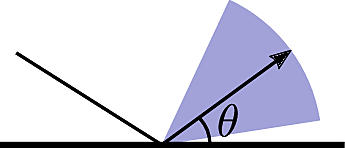
\includegraphics[width=0.6\linewidth]{img/bounce_example_nondet.jpg}
    \centering
    \caption[test]{\label{fig:bounce_def} Definition of an action $\theta$
taken when the robot encounters an environment boundary. The cone indicates the
type of uncertainty that we allow in our model.}
\end{figure}

This reorientation can be
implemented in various ways; yaw control combined with sensors (ie: scanners)
that can identify the boundary orientation relative to the robot, or even
mechanically (imagine a robot which aligns a planar body part to the wall, and
rotates the rest of its body to the desired heading). Our work focuses on the
high-level plans, assuming this reorientation can be executed somewhat reliably.

\section{Combinatorial Reasoning}

Since we assume the robots move in straight lines (with some possible
uncertainty in heading), our planner first discretizes the polygon boundary using {\em
visibility events}, points on the boundary where edges of the polygon pass in
and out of visibility as the robot slides along the boundary.
This approach allows us to compute a roadmap of
all the {\em safe} transitions (where any two points on a given segment along the
boundary can transition to the same edge under a set of actions). For
more details on this discretization, see \cite{nilles2018visibility}. This
planner can be used to generate paths that are safe under 
uncertainty in actuation, and is able to report the action set required at each
stage in the plan. A robot with some intrinsic error (such as shown in Figure
1) should then aim at the center of this set at each stage. However, by including dynamical 
information into this roadmap, we can improve the
completeness and robustness of the planner.

\section{Useful Dynamical Properties}

We define the dynamical system $f: \partial P \times U \to \partial P$ which is
the geometrically determined mapping between points on the boundary.
In polygons, the resulting dynamical system is a piecewise function, with a
different form for each pair of mutually visible edges. Sometimes, transitions
between straight-line boundaries have the property of {\em
contraction}: if the same action is taken from two different points, the
distance between the next locations is smaller than the distance between the
start points.

\begin{figure}
    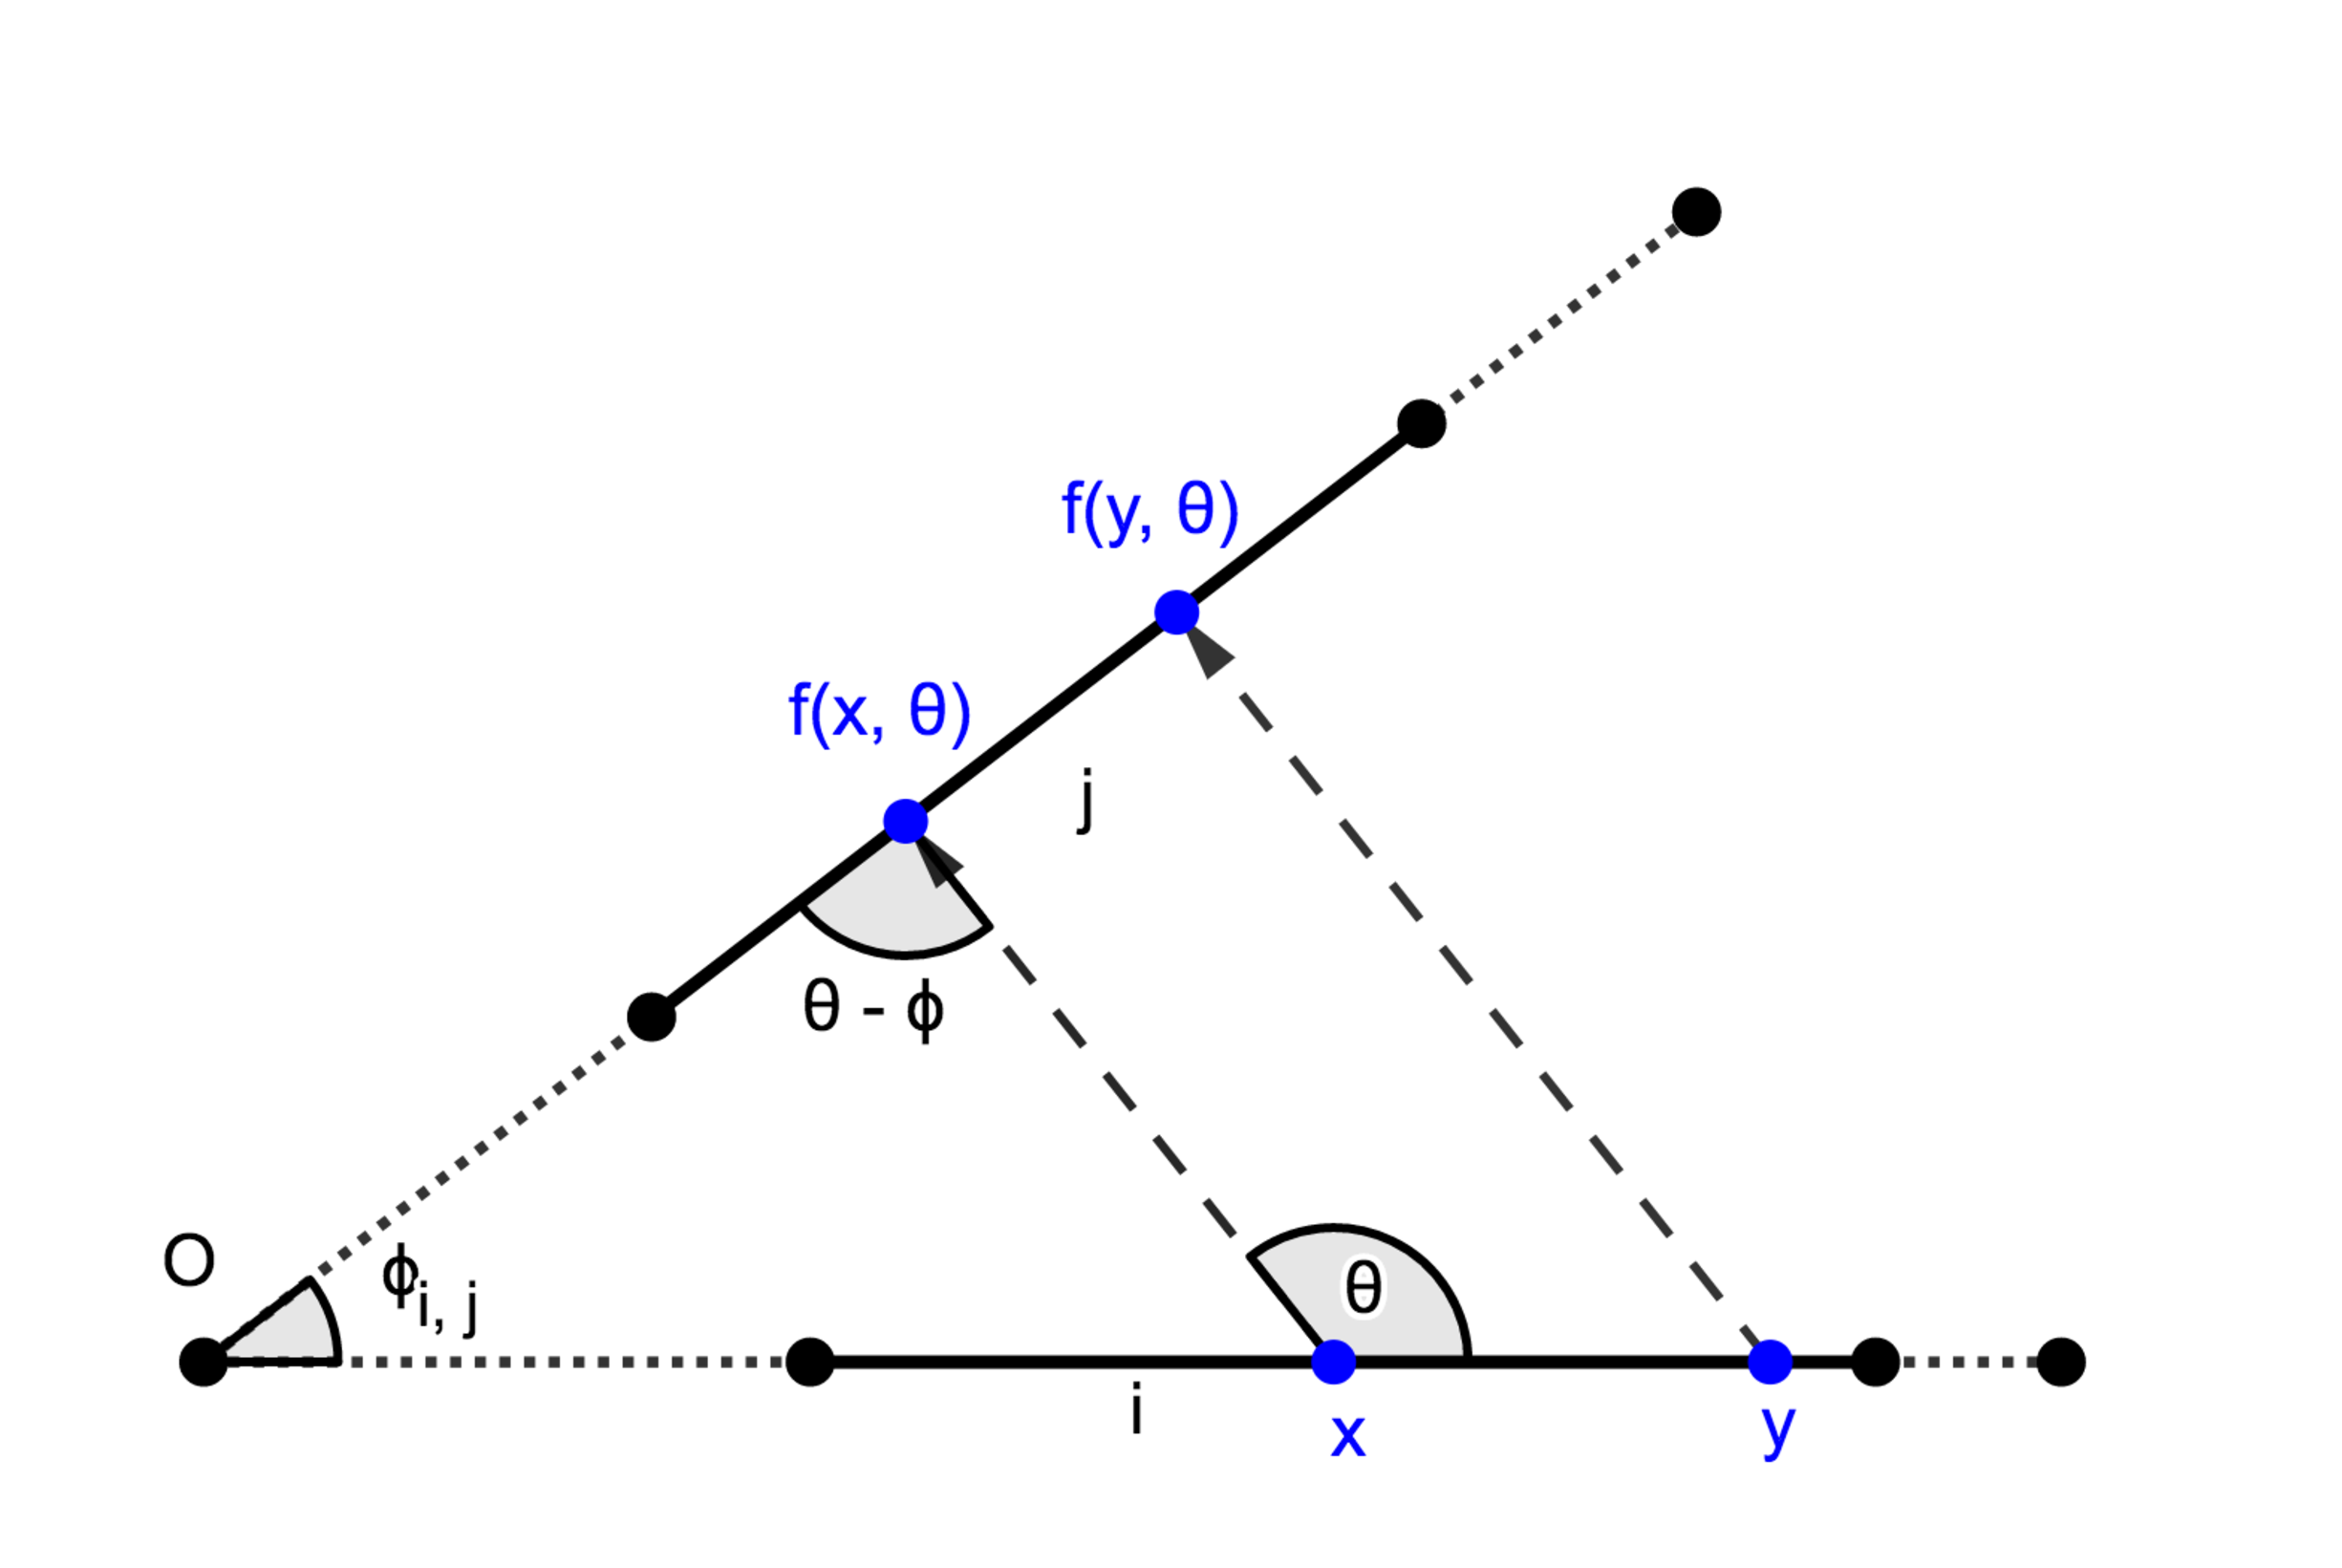
\includegraphics[width=0.8\linewidth]{img/contraction_map_cond.pdf}
    \centering
    \caption[test]{\label{fig:contraction_setup} The geometric set-up for
calculating the contraction coefficients between two line segments (solid black
segments). The robots start on the lower,
horizontal segment, indexed by $i$. They are transitioning under angle $\theta$
to edge $j$. Edges $i$ and $j$ have an internal angle of $\phi_{i,j}$.}
\end{figure}

We define a {\em contraction coefficient} for each pair of mutually visible edges in the
polygonal environment
as $c(\theta, i,j) = \frac{|f(x,\theta) - f(y,\theta)|}{|x-y|}$,
where $f$ is a contraction mapping if $c(\theta, i,j)$
is less than one. Using geometric reasoning, this contraction coefficient is calculated
to be \footnote{The type of the operator in the denominator depends on if the segments
would intersect on the right or the left of segment $i$ (in the case where the lines are parallel, $c(\theta, i,j) = 1$
always).}

$$
c(\theta, i,j) = \frac{\sin(\theta)}{\sin(\theta \pm \phi_{i,j})}.
$$
See Figure \ref{fig:contraction_setup} for an example of the geometric
scenario.

It is also important to note that $f$ is linear in $x$, so when transitions are
composed together, the contraction coefficient of the overall transition is the
product of the individual transitions. This lets us construct trajectories which
may have individual steps that allow the set of possible
robot locations to grow, but that are overall robust and reduce uncertainty.

To plan while taking these properties into account, we can compute a further
discretization of the polygon boundary. We are currently finely discretizing $\theta$ and
storing the contraction coefficients along the environment boundary in the roadmap. However, 
this leads to a large branching factor in the search for plans. We
are currently implementing a method where we compute values of $\theta$ that
cause combinatorial
changes in the resulting discretization ({\em critical angles}, as defined in
\cite{ErLav13}), and planning over actions that are not near critical angles,
decreasing the sensitivity of resulting strategies to modelling errors.

\section{Task-Motion Primitives}

Our understanding of the dynamics of these systems is developed to the point
where we can easily compute reachable sets and long-term dynamical behaviors of
different strategies. To make these systems more generally useful, 
we are developing some higher-level utilities for our planning
tool. For example, we may wish for a robot to repeatedly visit a few different regions of the
environment, or we may wish
to generate strategies that only use a few different bounce actions (for
mechanical designs in micro-scale settings). The first is a {\em spatial} task,
and the second is a {\em behavioral constraint}, and these types of tasks and constraints
can be combined.

Generally this is accomplished with different types of
searches in the generated roadmap. For example, we can label sections of the roadmap with
different ``colors" and using a search algorithm to find safe plans which visit
each region. Algorithms such as $A^*$ search can be used to find sequences of
transitions which are optimally contracting (maximally reduce uncertainty in robot
position and effect of nondeterminism). We can also search for strategies which
use maximally large nondeterministic actions, which allow for strategies which
are maximally tolerant of nondeterminism. The constraint of only using
one or a few bounce angles is again a type of search, where the interval of
bounce angles that will admit a path is updated at each transition and the
search path is abandoned if the interval becomes empty.

\section{Future Work}

We are in active development of an interactive interface which allows user to specify or
import polygonal maps and design different types of trajectories using a small
API which defines spatial tasks and behavioral constraints \footnote{see
\url{https://github.com/alexandroid000/bounce_viz} for more documentation}.

Additionally, some interesting theoretical questions remain which may impact more
general classes of problems. The contraction property described in this work holds not only in the two
dimensional setting. In three dimensions, for example, similar conditions can be
described for straight-line paths between two planar boundaries. We are
developing the theory for more general cases and are interested
in how our approach of making principled, geometric discretizations combined with
dynamical classification of transitions can be applied in more general settings.
 
\section*{Acknowledgments}

We would like to acknowledge Israel Becerra and Samara Ren for their
significant contributions to the project.

\bibliographystyle{plainnat}
\bibliography{refs}

\end{document}


